\documentclass[11pt,a4paper]{article}
\usepackage[spanish,activeacute]{babel}
\decimalpoint
\usepackage[utf8]{inputenc}
\usepackage{listingsutf8}
\usepackage{amsmath}
\usepackage{amsfonts}
\usepackage{amssymb}
\usepackage{graphicx}
\usepackage{color}
\usepackage{listings}
\usepackage{amsthm}
\usepackage{caption}
\usepackage{subcaption}
\usepackage{dsfont}
\usepackage{comment}
\usepackage{enumerate}
\usepackage{mathtools,xparse}
\usepackage{ mathrsfs }
\usepackage{float}
\usepackage{listings}
\usepackage{xcolor}
\usepackage[ruled]{algorithm2e}

%% CODIGO PYTHON
\definecolor{codegreen}{rgb}{0,0.6,0}
\definecolor{codegray}{rgb}{0.5,0.5,0.5}
\definecolor{codepurple}{rgb}{0.58,0,0.82}
\definecolor{backcolour}{rgb}{0.93,0.93,0.93}

\lstdefinestyle{mystyle}{
    backgroundcolor=\color{backcolour},   
    commentstyle=\color{codegreen},
    keywordstyle=\color{magenta},
    numberstyle=\tiny\color{codegray},
    stringstyle=\color{codepurple},
    basicstyle=\ttfamily\footnotesize,
    breakatwhitespace=false,         
    breaklines=true,                 
    captionpos=b,                    
    keepspaces=true,                 
    numbers=left,                    
    numbersep=5pt,                  
    showspaces=false,                
    showstringspaces=false,
    showtabs=false,                  
    tabsize=2
}

\lstset{style=mystyle, inputencoding=utf8, extendedchars=true, literate={á}{{\'a}}1 {ó}{{\'o}}1 {é}{{\'e}}1 {ú}{{\'u}}1 {í}{{\'i}}1 {ñ}{{\~n}}1,}
%CODIGO PYTHON
\usepackage[left=2.3cm, right=2.1cm, top=2.35cm, bottom=2.35cm]{geometry}
%\renewcommand{\rmdefault}{mathpazo}
%\usepackage{mathpazo}

\usepackage[]{hyperref}
\hypersetup{
    pdftitle={Práctica 3 - MH},
    pdfauthor={Mario Muñoz Mesa},
    pdfsubject={ },
    pdfkeywords={keyword1, keyword2},
    bookmarksnumbered=true,     
    bookmarksopen=true,         
    bookmarksopenlevel=1,       
    colorlinks=true,   
    linkcolor=black,         
    pdfstartview=Fit,           
    pdfpagemode=UseOutlines,
    pdfpagelayout=TwoPageRight
}


\DeclarePairedDelimiter{\norm}{\lVert}{\rVert}
\NewDocumentCommand{\normL}{ s O{} m }{%
  \IfBooleanTF{#1}{\norm*{#3}}{\norm[#2]{#3}}_{L_2(\Omega)}%
}

\DeclareMathOperator*{\argmax}{arg\,max}
\DeclareMathOperator*{\argmin}{arg\,min}

\newtheorem{theorem}{Teorema}

\theoremstyle{definition}
\newtheorem{definition}{Definición}[section]


\newtheorem{proposition}{Proposición}[section]


\newtheorem{corolary}{Corolario}[section]


\newtheorem{lema}{Lema}[section]

	\newcommand{\R}{\mathbb{R}}
	\newcommand{\N}{\mathbb{N}}
	\newcommand{\C}{\mathbb{C}}


\title{
\normalfont \normalsize 
\textsc{\small METAHEURÍSTICAS} \\ [10pt]
	
	
\huge{\textbf{Práctica 3 - APC}}\\

\textsc{\small Grupo 1} \\ [10pt]

	}

\author{Mario Muñoz Mesa\\ mario43514@correo.ugr.es}
\date{\today}


\begin{document}
	\maketitle
	\newpage
	\renewcommand*\contentsname{Índice}	
	\tableofcontents
	
	\newpage
	
	\section{Descripción del problema.}
	Nos ocupamos del problema del Aprendizaje de Pesos en Características (APC). Plantea, en el contexto de un problema de clasificación, elegir o ajustar un vector de pesos $\textbf{w}=(w_1,\ldots, w_d)\in [0,1]^d$ asociado a las características en base a un criterio de mejora del clasificador. Hemos denotado con $d$ al número de características.\\
	
	En nuestro caso trabajaremos con clasificador tipo 1-NN, y el criterio será maximizar:
	$$F(\textbf{w}):=\alpha\cdot \text{tasa\_clas}(\textbf{w})+(1-\alpha ) \cdot \text{tasa\_red}(\textbf{w})$$
	donde
	$$\text{tasa-clas}:=100\frac{\text{nº instancias bien clasificadas en training}}{\text{nº instancias en training}}, \quad \quad \text{tasa-red}:=100\frac{\text{nº valores } w_i <0.2}{\text{nº características}}$$
	y $alpha=0.5$ que pondera la importancia entre el acierto y la reducción de características para el nuevo mejor clasificador que se pretende encontrar.\\
	
	De lo que nos ocupamos por tanto es de obtener $\argmax_{\textbf{w}\in [0,1]^d} F(\textbf{w})$ para un clasificador 1-NN que utilizará la distancia ponderada
	$$d_{\textbf{w}}(u,v)=\sqrt{\sum_{i=1}^d w_i(u_i-v_i)^2}, \quad u,v\in \R^d$$
	para clasificar. Queremos que aumente el acierto y reduzca el número de características, cualquier característica con peso menor estricto a 0.2 se descarta.
	
	
	\newpage
	\section{Descripción de la aplicación de los algoritmos empleados.}
	\subsection{Asociados al preprocesado y representación. P1.}
	Partimos de un conjunto de entrenamiento $T$ formado por instancias de una muestra. Cada instancia se ha representado mediante una estructura de datos \texttt{SampleElement} que recoge las valores de las características en un vector \texttt{vector<double>} y la clase como una cadena de caracteres.
	
	De esta forma, cada dataset se lee mediante la función \texttt{read\_arff} y lo almacenamos como un vector de elementos muestrales \texttt{vector<SampleElement>}. 
	
	Para la normalización utilizamos min-max normalization, se ha implementado en \texttt{normalization}.
	
	Las particiones para la validación cruzada $k-fold$ se realizan respetando la proporción de clases en cada partición, para ello cada elemento de una clase se va asignando a una partición de forma cíclica.
	
	La solución será un vector de pesos con valores entre 0 y 1, cada componente indica el peso de una característica, se representa como un \texttt{vector<double>}
	\subsection{Asociados al preprocesado y representación. P3.}
	Para los algoritmos de Búsquedas basadas en Trayectorias se ha decidido crear una estructura, \texttt{Solution}, que contiene un \texttt{vector<double>} con el vector de pesos y su fitness asociado. 
	
	Además se han definido los comparadores mayor, $>$, y menor, $<$. Una solución es mayor a otra si su función objetivo es mayor, y menor si la función objetivo es menor.
	
	\subsection{Funciones generales. P1.}
	Nuestro clasificador utiliza la distancia euclídea, para manejarla se han implementado dos funciones: \texttt{euclidean\_distance2} y \texttt{euclidean\_distance2\_w}.\\
	
	
	\begin{algorithm}[H]
		\caption{euclidean\_distance2}
		\KwIn{vector de reales $a$, vector de reales $b$}
		\KwOut{la distancia euclídea al cuadrado entre $a$ y $b$}
		\Begin{
			dist $\leftarrow$ 0
			
			\For { $i=0$ to $a.size()-1$ }{
				dist $\leftarrow$ dist + $(a[i]-b[i])^2$
			}
			\Return dist
		}
	\end{algorithm}~\\
	
	\begin{algorithm}[H]
		\caption{euclidean\_distance2\_w}
		\KwIn{vector de reales $a$, vector de reales $b$, vector de pesos $weights$}
		\KwOut{la distancia euclídea ponderada y al cuadrado entre $a$ y $b$}
		\Begin{
			dist $\leftarrow$ 0
			
			\For { $i=0$ \textbf{to} $a.size() -1$ }{
			\tcp{se descartan las características con peso < 2}	
				\If{$weights[i] \geq 0.2$}{ 
				dist $\leftarrow$ dist + $(a[i]-b[i])^2$
				}
			}
			\Return dist
		}
	\end{algorithm}~\\
	
	La función \texttt{euclidean\_distance2}  se utiliza exclusivamente para el cálculo de amigo y enemigo más cercano en el algoritmo Relief. Con \texttt{euclidean\_distance2\_w} calculamos la distancia ponderada descartando pesos menores a 0.2, se utiliza en 1-NN y Búsqueda Local.
	
	En ambos casos calculamos la distancia euclídea al cuadrado por motivos de eficiencia y porque lo que nos interesa es comparar distancias, y como la raíz cuadrada es una función creciente, si $a>b$ $\Rightarrow $ $\sqrt{a}>\sqrt{b}$, no hay inconveniente en trabajar con la distancia al cuadrado.
	
	El algoritmo 1-NN, haciendo uso de distancia ponderada, se ha implementado en \texttt{one\_NN}.\\
	
	\begin{algorithm}[H]
		\caption{one\_NN}
		\KwIn{elemento muestral $sam\_el$ a clasificar, conjunto de elementos muestrales sobre el que buscar el más cercano $sam\_elements$, vector de pesos $weights$}
		\KwOut{la clase o etiqueta del elemento más cercano, $min\_l$}
		\Begin{
			$min\_dist \leftarrow \infty$
			
			\For { $e$ \textbf{in} $sam\_elements$ }{
				$d\leftarrow$ euclidean\_distance2\_w(e.features, sam\_el.features, weights)
				
				\If{$d < min\_dist$}{
					$min\_l$ $\leftarrow$ e.label\\
					$min\_dist \leftarrow d$
				}
			}
			\Return min\_l
		}
	\end{algorithm}~\\
	
	La versión con leave-one-out, que se utiliza en Búsqueda Local, simplemente consiste en dejar un elemento fuera. \\
	
	\begin{algorithm}[H]
		\caption{one\_NN\_lo}
		\KwIn{elemento muestral $sam\_el$ a clasificar, conjunto de elementos muestrales sobre el que buscar el más cercano $sam\_elements$, vector de pesos $weights$, posición de elemento a dejar fuera $leave\_out$}
		\KwOut{la clase o etiqueta del elemento más cercano, $min\_l$}
		\Begin{
			$min\_dist \leftarrow \infty$
			
			\For { $i=0$ \textbf{to} $sam\_elements.size()-1$ }{
			\If{$i\neq leave\_out$}{
				$d\leftarrow$ euclidean\_distance2\_w(sam\_elements[i].features, sam\_el.features, weights)
				
				\If{$d < min\_dist$}{
					$min\_l$ $\leftarrow$ sam\_elements[i].label\\
					$min\_dist \leftarrow d$
				}
			}
			}
			\Return min\_l
		}
	\end{algorithm}
	
	\subsection{Funciones generales. P3.}
	
	Para evaluar la función objetivo asociada a los pesos de una solución y asignarlo a la solución se ha creado la función \texttt{obj\_to\_solution}:\\
		
		\begin{algorithm}[H]
		\caption{obj\_to\_solution}
		\KwIn{solución $s$, vector de elementos muestrales $training$}
		\Begin{
		
		\For{$i=0$ \textbf{to} $training.size()$}{
			$class\_labels.push\_back(\ one\_NN\_lo(training[i], training, s.w, i)\ )$
		}
		
		$s.obj \leftarrow obj\_function(class\_rate(class\_labels, training), \ red\_rate(s.w))$
		}
	\end{algorithm}~\\
	
	El operador de mutación coincide con el de generación de vecinos en la BL, introduce una perturbación con una normal de media y desviación típica dadas por el argumento $n\_dist$. La media es 0 en todos los algoritmos y respecto a la desviación típica: en BL y ES es 0.3, y en ILS 0.4.  \\
	
	\begin{algorithm}[H]
		\caption{mutation}
		\KwIn{vector de pesos $weights$, índice a mutar $i$, distribución normal $n\_dist$}
		\Begin{
		$weights[i] \leftarrow weights[i] + e\in n\_dist$\\
		\If{$weigths[i]>1$}{
			$weights[i]\leftarrow 1$		
		}
		\Else{
			\If{$weights[i]<0$}{
				$weights[i]\leftarrow 0$			
			}		
		}
		}
	\end{algorithm}~\\
	
		La búsqueda local que es utilizada por BMB e ILS sigue el mismo esquema que en la práctica 1. Ahora sin embargo: se adapta a la estructura de solución definida, el número máximo de evaluaciones es 1000, y comenzará a partir de una solución dada como argumento, esta solución acabará conteniendo la solución resultante de la búsqueda local.\\
		
		\begin{algorithm}[H]
		\caption{local\_search}
		\KwIn{conjunto de elementos muestrales $training$, solución $sol$}
		\Begin{
			$n\leftarrow num\_feats$
		
			$max\_gen\_neighbours \leftarrow 20*n$
			
			$max\_objf\_evals \leftarrow 1000$			
			
			
			
			$new\_best\_obj \leftarrow false$
			
			$mod\_pos \leftarrow 0$
			
			$gen\_neighbours, \ obj\_eval\_count \leftarrow 0,\ 0$
			
			\tcp{se inicializan índices de las componentes}
			\For{$i=0$ \textbf{to} $n-1$}{
				$comp\_indexes.push\_back(i)$
			}
			
			$best\_obj \leftarrow sol.obj$\\ ~\\
			
			\While{$gen\_neighbours < max\_gen\_neighbours$ \textbf{and} $obj\_eval\_count < max\_objf\_evals$}{
			\tcp{aleatorizamos componentes a mutar si se han recorrido todas o se mejoró f.obj}
			\If{$new\_best\_obj$ \textbf{or} $mod\_pos \% n == 0$}{
				$new\_best\_obj \leftarrow false$\\
				$shuffle(comp\_indexes)$\\
				$mod\_pos \leftarrow 0$
			}
			\tcp{Se toma componente a mutar y se muta}
			$comp\_to\_mut \leftarrow comp\_indexes[mod\_pos \% n]$
			
			$muted\_sol\leftarrow sol$
			
			$mutation(muted\_sol.w,\ comp\_to\_mut,\  \mathcal{N}(0,\ 0.3))$
			
			$gen\_neighbours \leftarrow gen\_neighbours +1$
			
			\tcp{se asigna función objetivo a solución con los pesos mutados}
			$obj\_to\_solution(muted\_sol,\ training)$\\
			\tcp{Si se ha mejorado, actualizamos mejor objetivo y weights, y vecinos generados}
			\If{$muted\_sol.obj>best\_obj$}{
				$sol \leftarrow muted\_sol$\\
				$best\_obj \leftarrow sol.obj$\\
				$gen\_neighbours \leftarrow 0$\\
				$new\_best\_obj \leftarrow true$
			}
			
			$obj\_eval\_count\leftarrow obj\_eval\_count+1$\\
			$mod\_pos\leftarrow mod\_pos +1$
			}
				
		}
		
	\end{algorithm}~\\
		

	
	

	
	\subsection{Función objetivo.}
	Para el cálculo de las tasas se han implementado las funciones \texttt{class\_rate} y \texttt{red\_rate} que simplemente implementan la propia de definición de tasa-class y tasa-red.\\
	
	\begin{algorithm}[H]
		\caption{class\_rate}
		\KwIn{vector con clases o etiquetas de elementos clasificados $class\_labels$, elementos de test $test$}
		\KwOut{el porcentaje de acierto}
		\Begin{
			$n\leftarrow 0$\\
  			$class\_labels\_s \leftarrow class\_labels.size()$
  			
			\For { $i=0$ \textbf{to} $class\_labels\_s-1$ }{
			\If{$class\_labels\_s[i] == test[i].label$}{
				$n\leftarrow n+1$
			}

			}
			
			\Return $100\frac{n}{class\_labels\_n}$
		}
	\end{algorithm}~\\
	
	\begin{algorithm}[H]
		\caption{red\_rate}
		\KwIn{vector de pesos $weights$}
		\KwOut{el porcentaje de reducción}
		\Begin{
			$feats\_reduced \leftarrow 0$
			
			\For { $w$ \textbf{in} $weights$ }{
			\If{$w < 0.2$}{
				$feats\_reduced \leftarrow feats\_reduced+1$
			}

			}
			
			\Return $100\frac{feats\_reduced}{initial\_number\_of\_features}$
		}
	\end{algorithm} ~\\
	
	La función objetivo, teniendo en cuenta que trabajamos con $\alpha = 0.5$, nos quedaría:\\
	
	\begin{algorithm}[H]
		\caption{obj\_function}
		\KwIn{tasa de clasificación $class\_rate$, tasa de reducción $red\_rate$}
		\KwOut{el valor de la función objetivo o fitness}
		\Begin{
			
			\Return $\alpha \cdot class\_rate + (1-\alpha) \cdot red\_rate$
		}
	\end{algorithm}
	
	\section{Descripción de los algoritmos.}
	\subsection{Enfriamiento simulado (ES).}
	Este algoritmo es un algoritmo de búsqueda por trayectorias simple. Persigue además no quedar atrapado en óptimos locales. 
	
	Para ello parte de una ``temperatura'' inicial que irá disminuyendo conforme aumentan las iteraciones. Esta temperatura irá determinando la probabilidad de aceptar soluciones peores que la actual, a menor temperatura menor probabilidad de aceptar. De este modo, cuando la temperatura es muy baja (cercana a la final) la probabilidad de aceptar una solución peor es muy baja, y cuando al temperatura es alta (al comienzo) se aceptarán bastantes soluciones peores, incentivando la exploración.
	
	El operador de movimiento será la mutación normal con $\mu =0$ y $\sigma = 0.3$. En nuestro caso una solución mutada, $s_m$, de la solución actual, $s$, será aceptada si se cumple una de las dos condiciones:
	\begin{itemize}
	\item $\Delta f< 0 $ donde $\Delta f:=fitness(s) - fitness(s_m)$, pues nuestro problema es de maximización.
	\item Se verifica $u<e^{-\frac{\Delta f}{T\cdot K}}$ con $u\in U(0,1)$, donde $T$ es la temperatura actual y $K=1$.
	
	\textit{Nota:} en el caso de $\Delta f=0$, se toma $\Delta f = 2.5\cdot T_f$, donde $T_f$ es la temperatura final, de modo que conforme disminuya $T$, acercándose a $T_f$, menor será la probabilidad de aceptar una solución con mismo fitness que la actual. Cuando $T=T_f$ la probabilidad sería 0.082 (8.2\%). 
	\end{itemize}
	Adicionalmente, por cada mutación aceptada se comprueba si es la mejor solución hasta el momento, si lo es se guarda como la mejor.\\
	
	Para el enfriamiento de la temperatura se emplea el esquema de Cauchy modificado:
	$$T_{k+1}=\frac{T_k}{1+\beta \cdot T_k} \quad ; \quad \beta=\frac{T_0-T_f}{M\cdot T_0 \cdot T_f}$$
	donde $M$ es el número de enfriamientos a realizar, $T_0$ la temperatura inicial y $T_f$ la final. En nuestro caso:
	
	$$M=\frac{15000}{\text{máx\_vecinos}} \ ; \quad T_0=\frac{0.3\cdot fitness(s_0)}{-\ln(0.3)}\ ; \quad T_f=0.001 $$
	Donde $\text{máx\_vecinos} = 10 n$ donde $n$ es el tamaño del vector de pesos. 
	
	\textit{Nota:} como la temperatura inicial debe ser menor que la final se comprobará que sea así, en caso contrario se ha decidido reducir con $T_f=0.1\cdot T_f$ hasta que se cumpla.\\
	
	Se enfriará la temperatura cada vez que se generen máx\_vecinos o cada vez que se acepten $\text{máx\_éxitos}:=0.1\cdot \text{máx\_vecinos}$ vecinos.
	
	La condición de parada es alcanzar 15000 evaluaciones de la función objetivo o bien no haber logrado ningún éxito en el enfriamiento.
	
	
	El pseudocódigo es el siguiente:\\
	
	\begin{algorithm}[H]
		\caption{sim\_annealing}
		\KwIn{vector de elementos muestrales $training$}
		\KwOut{el vector de pesos de la mejor solución encontrada}
		\Begin{
			$max\_neighbours \leftarrow 10*n$
			
			$max\_success \leftarrow 0.1 * max\_neighbours$
			
			$max\_evals \leftarrow 15000$
			
			$evals,\ gen\_neighbours,\ num\_success \leftarrow 0,\ 0,\ 0$			
		
			$max\_anns \leftarrow max\_evals / max\_neighbours$
			
			$T_f \leftarrow 0.001$
			
			\tcp{Solución inicial}
			\For{$i=0$ \textbf{to} $n$}{
				$sol.w.push\_back(e\in U(0,1))$
			}
			$obj\_to\_solution(sol, training)$
			
			$evals\leftarrow 1$
			
			$best\_sol \leftarrow sol$

			$T_0\leftarrow 	\frac{0.3\cdot best\_sol.obj}{-\ln(0.3)}	$
			
			$T\leftarrow T_0$
			
			\While(\tcp*[h]{Temperatura final debe ser menor que la inicial}){$T_f \geq T$}{
				$T_f \leftarrow T_f * 0.1$
			}
			
			$\beta \leftarrow \frac{T_0-T_f}{max\_anns \cdot T_0 \cdot T_f}$
			
			$num\_success \leftarrow -1$
			
			\While{$evals < max\_evals$ \textbf{and} $num\_success \neq 0$}{
				$gen\_neighbours \leftarrow 0$
				
				$num\_success \leftarrow 0$
				
				\While{$evals < max\_evals$ \textbf{and} $gen\_neighbours < max\_neighbours$ \textbf{and} $num\_success < max\_success$}{
					$muted\_sol \leftarrow sol$
					
					$mutation(muted\_sol.w, rand(0,n-1), \mathcal{N}(0,0.3))$
					
					$obj\_to\_solution(muted\_sol, training)$
					
					$evals \leftarrow evals+1$
					
					$gen\_neighbours \leftarrow gen\_neighbours +1 $
					
					$\Delta f \leftarrow sol.obj - muted\_sol.obj$
					
					\tcp{Si tienen mismo fitness también se controla que la probabilidad de aceptar vaya disminuyendo con la temperatura}
					\If{$\Delta f == 0$}{
						$\Delta f \leftarrow 2.5 * T_f$
					}
					\If{$\Delta f < 0$ \textbf{or} $rand(0,1) \leq e^{-\frac{\Delta f}{T}}$}{
						$num\_success \leftarrow num\_success +1$
						
						$sol \leftarrow muted\_sol$
						
						\If{$sol.obj > best\_sol.obj$}{
							$best\_sol \leftarrow sol$
						}
					}
				}
				$T\leftarrow \frac{T}{1+\beta * T}$
			}
			
			\Return $best\_sol.w$
		}
	\end{algorithm}
	\subsection{Búsqueda Multiarranque Básica (BMB).}
	El algoritmo BMB consiste en aplicar BL a varias soluciones generadas aleatoriamente, guardando las obtenidas tras al BL y devolviendo la mejor.
	
	En nuestro caso se generarán 15 soluciones aleatorias, cada BL local aplicada realizará un máximo de 1000 evaluaciones de la función objetivo.\\
	
	\begin{algorithm}[H]
		\caption{bmb}
		\KwIn{vector de elementos muestrales $training$}
		\KwOut{el vector de pesos de la mejor solucion encontrada}
		\Begin{
			$max\_its \leftarrow 15$
			
			$best\_sol.obj \leftarrow -1$
			
			\For{$i=0$ \textbf{to} $max\_its-1$}{
				\tcp{solución aleatoria}
				\For{$j=0$ \textbf{to} $n-1$}{
					$sol.w[j] \leftarrow u\in U(0,1)$
				}
				
				$obj\_to\_solution(sol,training)$
				
				$local\_search(training, sol)$
				
				\If{$sol.obj > best\_sol.obj$}{
					$best\_sol \leftarrow sol$
				}
			}
			
			\Return{$best\_sol.w$}
		
		}
			
	\end{algorithm}
	
	
	\subsection{Búsqueda Local Reiterada (ILS).}
	El algoritmo ILS consistirá en generar una solución inicial aleatoria y aplicar el
algoritmo de BL sobre ella. Una vez obtenida la solución optimizada, se estudiará si es
mejor que la mejor solución encontrada hasta el momento y se realizará una mutación
sobre la mejor de estas dos, volviendo a aplicar el algoritmo de BL sobre esta solución
mutada. Este proceso se repite un determinado número de veces, devolviéndose la mejor
solución encontrada en todo el proceso.

	La mutación a aplicar consite en mutar conjuntamente $t=0.1\cdot n$ características aleatorias con el operador de mutación que venimos usando pero esta vez con $\sigma=0.4$.
	
	En total se realizarán 15 llamadas a BL, y cada BL realizará un máximo de 1000 evaluaciones de la función objetivo.\\

	 
	 \begin{algorithm}[H]
		\caption{ils}
		\KwIn{vector de elementos muestrales $training$}
		\KwOut{el vector de pesos de la mejor solucion encontrada}
		\Begin{
			$max\_its \leftarrow 15$

			$t \leftarrow round(0.1*n)$			
			
			\tcp{Solución inicial}
			\For{$i=0$ \textbf{to} $n-1$}{
				$sol.w.push\_back(e\in U(0,1))$
			}
			$obj\_to\_solution(sol, training)$
			
			\tcp{Índices a mutar}
			\For{$i=0$ \textbf{to} $n-1$}{
				$indexes.push\_back(i)$
			}
			
			$local\_search(training, sol)$
			
			\For{$i=1$ \textbf{to} $max\_its -1$}{
				$shuffle(indexes)$
				
				$muted\_sol \leftarrow sol$
				
				\For{$j=0$ \textbf{to} $t-1$}{
					$mutation(muted\_sol.w, indexes[j], \mathcal{N}(0,0.4))$
				}
				$obj\_to\_solution(muted\_sol, training)$
				
				$local\_search(training, muted\_sol)$
				
				\If{$muted\_sol.obj>sol.obj$}{
					$sol\leftarrow muted\_sol$
				}
			}
			\Return{$sol.w$}
		
		}
			
	\end{algorithm}
	
	\subsection{Algoritmo híbrido ILS-ES.}
		Este algoritmo sigue el mismo esquema que ILS a excepción de utilizar ES en lugar de BL.
		
		Para este algoritmo se adapta el pseudocódigo de ES para partir ya de una solución dada y realizar como máximo 1000 evaluaciones de la función objetivo (para que en total realice 15000 evaluaciones de función objetivo como el resto de algoritmos y sea equiparable)\\

		Pseudocódigo de ES adaptado:\\
		
	\begin{algorithm}[H]
		\caption{sim\_annealing\_s}
		\KwIn{vector de elementos muestrales $training$, solución de partida $s$}
		\KwOut{la mejor solución encontrada}
		\Begin{
			$max\_neighbours \leftarrow 10*n$
			
			$max\_success \leftarrow 0.1 * max\_neighbours$
			
			$max\_evals \leftarrow 1000$
		
			$max\_anns \leftarrow max\_evals / max\_neighbours$

			$evals,\ gen\_neighbours,\ num\_success \leftarrow 0,\ 0,\ 0$			
			
			$T_f \leftarrow 0.001$
			
			$sol\leftarrow s$
			
			
			$best\_sol \leftarrow sol$

			$T_0\leftarrow 	\frac{0.3\cdot best\_sol.obj}{-\ln(0.3)}	$
			
			$T\leftarrow T_0$
			
			
			\While(\tcp*[h]{Temperatura final debe ser menor que la inicial}){$T_f \geq T$}{
				$T_f \leftarrow T_f * 0.1$
			}
			
			$\beta \leftarrow \frac{T_0-T_f}{max\_anns \cdot T_0 \cdot T_f}$
			
			$num\_success \leftarrow -1$
			
			\While{$evals < max\_evals$ \textbf{and} $num\_success \neq 0$}{
				$gen\_neighbours \leftarrow 0$
				
				$num\_success \leftarrow 0$
				
				\While{$evals < max\_evals$ \textbf{and} $gen\_neighbours < max\_neighbours$ \textbf{and} $num\_success < max\_success$}{
					$muted\_sol \leftarrow sol$
					
					$mutation(muted\_sol.w, rand(0,n-1), \mathcal{N}(0,0.3))$
					
					$obj\_to\_solution(muted\_sol, training)$
					
					$evals \leftarrow evals+1$
					
					$gen\_neighbours \leftarrow gen\_neighbours +1 $
					
					$\Delta f \leftarrow sol.obj - muted\_sol.obj$
					
					\tcp{Si tienen mismo fitness también se controla que la probabilidad de aceptar vaya disminuyendo con la temperatura}
					\If{$\Delta f == 0$}{
						$\Delta f \leftarrow 2.5 * T_f$
					}
					\If{$\Delta f < 0$ \textbf{or} $rand(0,1) \leq e^{-\frac{\Delta f}{T}}$}{
						$num\_success \leftarrow num\_success +1$
						
						$sol \leftarrow muted\_sol$
						
						\If{$sol.obj > best\_sol.obj$}{
							$best\_sol \leftarrow sol$
						}
					}
				}
				$T\leftarrow \frac{T}{1+\beta * T}$
			}
			
			\Return $best\_sol$
		}
	\end{algorithm}~\\
	
	Con esta modificación el pseudocódigo de ILS-ES es exactamente igual que ILS pero sustituyendo las llamadas a \texttt{local\_search} por llamadas a \texttt{sim\_annealing\_s}.
	\section{Procedimiento considerado en el desarrollo.}
	Para el desarrollo de la práctica no se ha utilizado ningún framework, se han implementado las funciones necesarias en C++. Todo el código se encuentra en \texttt{p3.cpp} .
	
	Para la ejecución basta indicar un argumento con el archivo a ejecutar, en este caso se utiliza la semilla por defecto 1234, que es la misma que se utilizó para los resultados de esta memoria.
	
	También se incluye un fichero \texttt{p3\_all\_datasets.sh} que ejecuta, con la semilla por defecto, \texttt{p3} sobre los 3 datasets.
	
	\section{Experimentos y análisis de resultados.}
	Los 3 datasets con los que se ha trabajado son:
	\begin{itemize}
		\item \textbf{Ionosphere}: Conjunto de datos de radar que fueron recogidos por un sistema \textit{Goose Bay}, Labrador. Consta de 352 instancias con 34 características y 2 clases.
		\item \textbf{Parkinsons}: Conjunto de datos orientado a distinguir entre la presencia y ausencia de la enfermedad de Parkinson. Consta de 195 ejemplos con 22 características y 2 clases.
		\item \textbf{Spectf-Heart}: Conjunto de datos de detección de enfermedades cardiacas a partir de imágenes médicas de tomografía computerizada del corazón de pacientes. Consta de 267 ejemplos con 44 características y 2 clases.
	\end{itemize}
	
	Los resultados obtenidos son en 1-NN, BL y Relief fueron:~\\
	
		\textbf{1-NN}

	\begin{tabbing}
	\resizebox{\textwidth}{!}{%
		\begin{tabular}{|c|}
			\hline \textbf{Nº}\\ \textbf{part.} 
			\\ \hline
			\textbf{P1} \\ \hline 
			\textbf{P2} \\ \hline
			\textbf{P3} \\ \hline 
			\textbf{P4} \\ \hline
			\textbf{P5} \\ \hline
			\textbf{Media} \\ \hline
		\end{tabular}
		\begin{tabular}{|c|c|c|c|}
			\hline
			\multicolumn{4}{|c|}{\textbf{Ionosphere}} \\ \hline
			\textbf{\%clas} & \textbf{\%red} & \textbf{Agr.} & \textbf{T} \\ \hline 
			87.3239	&0	&43.662	&0.373 \\ \hline
64.2857	&0	&32.1429&	0.325 \\ \hline
64.2857	&0	&32.1429&	0.325 \\ \hline
64.2857	&0	&32.1429&	0.325 \\ \hline
64.2857	&0	&32.1429&	0.381 \\ \hline
68.89334	&0	&34.44672	&0.3458 \\ \hline
		\end{tabular}
		
		\begin{tabular}{|c|c|c|c|}
			\hline
			\multicolumn{4}{|c|}{\textbf{Parkinsons}} \\ \hline
			\textbf{\%clas} & \textbf{\%red} & \textbf{Agr.} & \textbf{T} \\ \hline 
95	      &0	&47.5	   & 0.181\\ \hline
25	      &0	&12.5	   & 0.073\\ \hline
25.641	  &0	&12.8205	&  0.072\\ \hline
23.6842	  &0	&11.8421	&  0.07\\ \hline
23.6842	  &0	&11.8421	&  0.071\\ \hline
38.60188	&0	&19.30094&	0.0934\\ \hline

		\end{tabular}
		
		\begin{tabular}{|c|c|c|c|}
			\hline
			\multicolumn{4}{|c|}{\textbf{Spectf-Heart}} \\ \hline
			\textbf{\%clas} & \textbf{\%red} & \textbf{Agr.} & \textbf{T} \\ \hline 
			85.7143	&0	&42.8571	&  0.468\\ \hline
72.8571	&0	&36.4286	&  0.407\\ \hline
72.8571	&0	&36.4286	&  0.397\\ \hline
72.8571	&0	&36.4286	&  0.397\\ \hline
73.5294	&0	&36.7647	&  0.388\\ \hline
75.563	&0	&37.78152&	0.4114\\ \hline

		\end{tabular}
		}
	\end{tabbing}
	
	\textbf{Relief}
	
		\begin{tabbing}
	\resizebox{\textwidth}{!}{%
		\begin{tabular}{|c|}
			\hline \textbf{Nº}\\ \textbf{part.} 
			\\ \hline
			\textbf{P1} \\ \hline 
			\textbf{P2} \\ \hline
			\textbf{P3} \\ \hline 
			\textbf{P4} \\ \hline
			\textbf{P5} \\ \hline
			\textbf{Media} \\ \hline
		\end{tabular}
		\begin{tabular}{|c|c|c|c|}
			\hline
			\multicolumn{4}{|c|}{\textbf{Ionosphere}} \\ \hline
			\textbf{\%clas} & \textbf{\%red} & \textbf{Agr.} & \textbf{T} \\ \hline 
			88.7324	&  2.94118&	45.8368	 & 1.753\\ \hline
			84.2857	&  5.88235&	45.084	  &1.757\\ \hline
			90    	 & 2.94118	&46.4706	  &1.76\\ \hline
			88.5714	&  2.94118&	45.7563	 & 1.761\\ \hline
			87.1429	&  2.94118&	45.042	  &1.766\\ \hline
			87.74648&	3.529414& 45.63794	&1.7594\\ \hline

		\end{tabular}
		
		\begin{tabular}{|c|c|c|c|}
			\hline
			\multicolumn{4}{|c|}{\textbf{Parkinsons}} \\ \hline
			\textbf{\%clas} & \textbf{\%red} & \textbf{Agr.} & \textbf{T} \\ \hline 
			95	      &9.09091	  &52.0455	  &0.364\\ \hline
97.5	    &4.54545	  &51.0227	  &0.366\\ \hline
94.8718	  &4.54545	  &49.7086	  &0.371\\ \hline
92.1053	  &4.54545	  &48.3254	  &0.369\\ \hline
100	      &0	        &50	        &0.374\\ \hline
95.89542	&4.545452	  &50.22044	  &0.3688\\ \hline
		\end{tabular}
		
		\begin{tabular}{|c|c|c|c|}
			\hline
			\multicolumn{4}{|c|}{\textbf{Spectf-Heart}} \\ \hline
			\textbf{\%clas} & \textbf{\%red} & \textbf{Agr.} & \textbf{T} \\ \hline 
			90	      &0	&45	      &2.28\\ \hline
87.1429	  &0	&43.5714	  &2.222\\ \hline
80	      &0	&40	      &2.201\\ \hline
84.2857	  &0	&42.1429	  &2.172 \\ \hline
77.9412	  &0	&38.9706	  &2.237 \\ \hline
83.87396	&0	&41.93698	&2.2224\\ \hline

		\end{tabular}
		}
	\end{tabbing}
	
	\textbf{Búsqueda Local (BL)}
	
		\begin{tabbing}
	\resizebox{\textwidth}{!}{%
		\begin{tabular}{|c|}
			\hline \textbf{Nº}\\ \textbf{part.} 
			\\ \hline
			\textbf{P1} \\ \hline 
			\textbf{P2} \\ \hline
			\textbf{P3} \\ \hline 
			\textbf{P4} \\ \hline
			\textbf{P5} \\ \hline
			\textbf{Media} \\ \hline
		\end{tabular}
		\begin{tabular}{|c|c|c|c|}
			\hline
			\multicolumn{4}{|c|}{\textbf{Ionosphere}} \\ \hline
			\textbf{\%clas} & \textbf{\%red} & \textbf{Agr.} & \textbf{T} \\ \hline 
			78.8732	&85.2941	&82.0837	  &3311.36\\ \hline
92.8571	&85.2941	&89.0756	  &4673.61\\ \hline
95.7143	&82.3529	&89.0336	  &1986.46\\ \hline
88.5714	&88.2353	&88.4034	  &3914.9\\ \hline
90	    &85.2941	&87.6471	  &2388.89\\ \hline
89.2032&	85.2941&	87.24868	&3255.044\\ \hline

		\end{tabular}
		
		\begin{tabular}{|c|c|c|c|}
			\hline
			\multicolumn{4}{|c|}{\textbf{Parkinsons}} \\ \hline
			\textbf{\%clas} & \textbf{\%red} & \textbf{Agr.} & \textbf{T} \\ \hline 
			87.5	 &86.3636	  &86.9318&	390.064\\ \hline
82.5	 &90.9091	  &86.7045&	408.803\\ \hline
87.1795	&86.3636	  &86.7716&	339.172\\ \hline
86.8421&	50	      &68.4211&	265.049\\ \hline
97.3684&	86.3636	 & 91.866&	581.204\\ \hline
88.278&	79.99998	&84.139	&396.8584\\ \hline

		\end{tabular}
		
		\begin{tabular}{|c|c|c|c|}
			\hline
			\multicolumn{4}{|c|}{\textbf{Spectf-Heart}} \\ \hline
			\textbf{\%clas} & \textbf{\%red} & \textbf{Agr.} & \textbf{T} \\ \hline 
			85.7143	 & 88.6364	&87.1753	 & 6719.91 \\ \hline
85.7143	&  86.3636&	86.039	 & 7458.06 \\ \hline
88.5714	 & 88.6364	&88.6039	 & 5512.85 \\ \hline
85.7143	 & 77.2727	&81.4935	 & 3448.21 \\ \hline
80.8824	 & 88.6364	&84.7594	 & 3612.81 \\ \hline
85.31934&	85.9091	&85.61422	&5350.368 \\ \hline
		\end{tabular}
		}
	\end{tabbing}
	
	Los resultados de ES, BMB, ILS e ILS-ES: ~\\
	
	\textbf{ES}
	
		\begin{tabbing}
	\resizebox{\textwidth}{!}{%
		\begin{tabular}{|c|}
			\hline \textbf{Nº}\\ \textbf{part.} 
			\\ \hline
			\textbf{P1} \\ \hline 
			\textbf{P2} \\ \hline
			\textbf{P3} \\ \hline 
			\textbf{P4} \\ \hline
			\textbf{P5} \\ \hline
			\textbf{Media} \\ \hline
		\end{tabular}
		\begin{tabular}{|c|c|c|c|}
			\hline
			\multicolumn{4}{|c|}{\textbf{Ionosphere}} \\ \hline
			\textbf{\%clas} & \textbf{\%red} & \textbf{Agr.} & \textbf{T} \\ \hline 
			84.507 & 88.2353 & 86.3712 & 22259 \\ \hline
84.2857 & 85.2941 & 84.7899 & 24425.6 \\ \hline
85.7143 & 85.2941 & 85.5042 & 25713.9 \\ \hline
85.7143 & 88.2353 & 86.9748 & 22850.6 \\ \hline
90 & 88.2353 & 89.1176 & 25145 \\ \hline
86.0443 & 87.0588 & 86.5515 & 24078.8 \\ \hline

		\end{tabular}
		
		\begin{tabular}{|c|c|c|c|}
			\hline
			\multicolumn{4}{|c|}{\textbf{Parkinsons}} \\ \hline
			\textbf{\%clas} & \textbf{\%red} & \textbf{Agr.} & \textbf{T} \\ \hline 
			87.5 & 86.3636 & 86.9318 & 4260.59 \\ \hline
87.5 & 86.3636 & 86.9318 & 4846.22 \\ \hline
84.6154 & 86.3636 & 85.4895 & 4339.23 \\ \hline
86.8421 & 90.9091 & 88.8756 & 4912.97 \\ \hline
89.4737 & 86.3636 & 87.9187 & 4296.52 \\ \hline
87.1862 & 87.2727 & 87.2295 & 4531.11 \\ \hline


		\end{tabular}
		
		\begin{tabular}{|c|c|c|c|}
			\hline
			\multicolumn{4}{|c|}{\textbf{Spectf-Heart}} \\ \hline
			\textbf{\%clas} & \textbf{\%red} & \textbf{Agr.} & \textbf{T} \\ \hline 
			77.1429 & 86.3636 & 81.7532 & 27566.4 \\ \hline
88.5714 & 84.0909 & 86.3312 & 24123.4 \\ \hline
90 & 86.3636 & 88.1818 & 28748.5 \\ \hline
82.8571 & 86.3636 & 84.6104 & 26001.8 \\ \hline
85.2941 & 84.0909 & 84.6925 & 29975.9 \\ \hline
84.7731 & 85.4545 & 85.1138 & 27283.2 \\ \hline
		\end{tabular}
		}
	\end{tabbing}
	
	\textbf{BMB}
	
		\begin{tabbing}
	\resizebox{\textwidth}{!}{%
		\begin{tabular}{|c|}
			\hline \textbf{Nº}\\ \textbf{part.} 
			\\ \hline
			\textbf{P1} \\ \hline 
			\textbf{P2} \\ \hline
			\textbf{P3} \\ \hline 
			\textbf{P4} \\ \hline
			\textbf{P5} \\ \hline
			\textbf{Media} \\ \hline
		\end{tabular}
		\begin{tabular}{|c|c|c|c|}
			\hline
			\multicolumn{4}{|c|}{\textbf{Ionosphere}} \\ \hline
			\textbf{\%clas} & \textbf{\%red} & \textbf{Agr.} & \textbf{T} \\ \hline 
			88.7324 & 88.2353 & 88.4838 & 21180.7 \\ \hline
84.2857 & 91.1765 & 87.7311 & 21030.1 \\ \hline
92.8571 & 85.2941 & 89.0756 & 21208.9 \\ \hline
87.1429 & 85.2941 & 86.2185 & 20306.1 \\ \hline
90 & 88.2353 & 89.1176 & 20431.2 \\ \hline
88.6036 & 87.6471 & 88.1253 & 20831.4 \\ \hline

		\end{tabular}
		
		\begin{tabular}{|c|c|c|c|}
			\hline
			\multicolumn{4}{|c|}{\textbf{Parkinsons}} \\ \hline
			\textbf{\%clas} & \textbf{\%red} & \textbf{Agr.} & \textbf{T} \\ \hline 
			87.5 & 86.3636 & 86.9318 & 4202.84 \\ \hline
100 & 81.8182 & 90.9091 & 4005.66 \\ \hline
94.8718 & 90.9091 & 92.8904 & 4504.04 \\ \hline
89.4737 & 81.8182 & 85.6459 & 4169.52 \\ \hline
92.1053 & 90.9091 & 91.5072 & 4418.87 \\ \hline
92.7901 & 86.3636 & 89.5769 & 4260.19 \\ \hline

		\end{tabular}
		
		\begin{tabular}{|c|c|c|c|}
			\hline
			\multicolumn{4}{|c|}{\textbf{Spectf-Heart}} \\ \hline
			\textbf{\%clas} & \textbf{\%red} & \textbf{Agr.} & \textbf{T} \\ \hline 
			87.1429 & 84.0909 & 85.6169 & 24765.9 \\ \hline
90 & 84.0909 & 87.0455 & 24605.9 \\ \hline
84.2857 & 81.8182 & 83.0519 & 24914.8 \\ \hline
88.5714 & 84.0909 & 86.3312 & 25037.6 \\ \hline
83.8235 & 90.9091 & 87.3663 & 25600 \\ \hline
86.7647 & 85 & 85.8824 & 24984.8 \\ \hline
		\end{tabular}
		}
	\end{tabbing}

	
	\textbf{ILS}
	
	\begin{tabbing}
	\resizebox{\textwidth}{!}{%
		\begin{tabular}{|c|}
			\hline \textbf{Nº}\\ \textbf{part.} 
			\\ \hline
			\textbf{P1} \\ \hline 
			\textbf{P2} \\ \hline
			\textbf{P3} \\ \hline 
			\textbf{P4} \\ \hline
			\textbf{P5} \\ \hline
			\textbf{Media} \\ \hline
		\end{tabular}
		\begin{tabular}{|c|c|c|c|}
			\hline
			\multicolumn{4}{|c|}{\textbf{Ionosphere}} \\ \hline
			\textbf{\%clas} & \textbf{\%red} & \textbf{Agr.} & \textbf{T} \\ \hline 
			87.3239 & 91.1765 & 89.2502 & 20627.8 \\ \hline
90 & 91.1765 & 90.5882 & 21020 \\ \hline
84.2857 & 88.2353 & 86.2605 & 19157.3 \\ \hline
85.7143 & 91.1765 & 88.4454 & 21414.7 \\ \hline
87.1429 & 91.1765 & 89.1597 & 18949.2 \\ \hline
86.8934 & 90.5882 & 88.7408 & 20233.8 \\ \hline

		\end{tabular}
		
		\begin{tabular}{|c|c|c|c|}
			\hline
			\multicolumn{4}{|c|}{\textbf{Parkinsons}} \\ \hline
			\textbf{\%clas} & \textbf{\%red} & \textbf{Agr.} & \textbf{T} \\ \hline 
			87.5 & 90.9091 & 89.2045 & 2451.35 \\ \hline
95 & 90.9091 & 92.9545 & 2840.84 \\ \hline
94.8718 & 90.9091 & 92.8904 & 2677.5 \\ \hline
89.4737 & 90.9091 & 90.1914 & 2462.07 \\ \hline
86.8421 & 90.9091 & 88.8756 & 2587.95 \\ \hline
90.7375 & 90.9091 & 90.8233 & 2603.94 \\ \hline

		\end{tabular}
		
		\begin{tabular}{|c|c|c|c|}
			\hline
			\multicolumn{4}{|c|}{\textbf{Spectf-Heart}} \\ \hline
			\textbf{\%clas} & \textbf{\%red} & \textbf{Agr.} & \textbf{T} \\ \hline 
			78.5714 & 90.9091 & 84.7403 & 26641.3 \\ \hline
90 & 93.1818 & 91.5909 & 27344.6 \\ \hline
87.1429 & 93.1818 & 90.1623 & 28861.9 \\ \hline
85.7143 & 93.1818 & 89.4481 & 27934.9 \\ \hline
82.3529 & 88.6364 & 85.4947 & 27081.3 \\ \hline
84.7563 & 91.8182 & 88.2872 & 27572.8 \\ \hline
		\end{tabular}
		}
	\end{tabbing}
	
	\textbf{ILS-ES}
	
	\begin{tabbing}
	\resizebox{\textwidth}{!}{%
		\begin{tabular}{|c|}
			\hline \textbf{Nº}\\ \textbf{part.} 
			\\ \hline
			\textbf{P1} \\ \hline 
			\textbf{P2} \\ \hline
			\textbf{P3} \\ \hline 
			\textbf{P4} \\ \hline
			\textbf{P5} \\ \hline
			\textbf{Media} \\ \hline
		\end{tabular}
		\begin{tabular}{|c|c|c|c|}
			\hline
			\multicolumn{4}{|c|}{\textbf{Ionosphere}} \\ \hline
			\textbf{\%clas} & \textbf{\%red} & \textbf{Agr.} & \textbf{T} \\ \hline 
			84.507 & 94.1176 & 89.3123 & 21557.7 \\ \hline
84.2857 & 91.1765 & 87.7311 & 24182.3 \\ \hline
88.5714 & 91.1765 & 89.8739 & 23002.1 \\ \hline
84.2857 & 91.1765 & 87.7311 & 22168.8 \\ \hline
82.8571 & 94.1176 & 88.4874 & 22922.7 \\ \hline
84.9014 & 92.3529 & 88.6272 & 22766.7 \\ \hline

		\end{tabular}
		
		\begin{tabular}{|c|c|c|c|}
			\hline
			\multicolumn{4}{|c|}{\textbf{Parkinsons}} \\ \hline
			\textbf{\%clas} & \textbf{\%red} & \textbf{Agr.} & \textbf{T} \\ \hline 
			87.5 & 86.3636 & 86.9318 & 4612.44 \\ \hline
85 & 90.9091 & 87.9545 & 4563.85 \\ \hline
94.8718 & 90.9091 & 92.8904 & 4446.55 \\ \hline
89.4737 & 90.9091 & 90.1914 & 4833.17 \\ \hline
94.7368 & 90.9091 & 92.823 & 4799.14 \\ \hline
90.3165 & 90 & 90.1582 & 4651.03 \\ \hline

		\end{tabular}
		
		\begin{tabular}{|c|c|c|c|}
			\hline
			\multicolumn{4}{|c|}{\textbf{Spectf-Heart}} \\ \hline
			\textbf{\%clas} & \textbf{\%red} & \textbf{Agr.} & \textbf{T} \\ \hline 
			78.5714 & 90.9091 & 84.7403 & 25224.6 \\ \hline
88.5714 & 88.6364 & 88.6039 & 26319.7 \\ \hline
80 & 90.9091 & 85.4545 & 26299.9 \\ \hline
87.1429 & 90.9091 & 89.026 & 27123.8 \\ \hline
85.2941 & 90.9091 & 88.1016 & 26896.5 \\ \hline
83.916 & 90.4545 & 87.1853 & 26372.9 \\ \hline
		\end{tabular}
		}
	\end{tabbing}
	
	
	Se muestra la tabla resumen:
	
	\begin{tabbing}
	\resizebox{\textwidth}{!}{%
		\begin{tabular}{|c|}
			\hline \textbf{Nº}\\ \textbf{part.} 
			\\ \hline
			\textbf{1-NN} \\ \hline 
			\textbf{Relief} \\ \hline
			\textbf{BL} \\ \hline 
			\textbf{ES} \\ \hline
			\textbf{BMB} \\ \hline
			\textbf{ILS} \\ \hline
			\textbf{ILS-ES} \\ \hline
		\end{tabular}
		\begin{tabular}{|c|c|c|c|}
			\hline
			\multicolumn{4}{|c|}{\textbf{Ionosphere}} \\ \hline
			\textbf{\%clas} & \textbf{\%red} & \textbf{Agr.} & \textbf{T} \\ \hline 
			68.89334	&0	          &34.44672	&0.3458\\ \hline
87.74648&	3.529414	  &45.63794	&1.7594\\ \hline
89.2032	  &85.2941	    &87.24868	&3255.044\\ \hline
86.0443 & 87.0588 & 86.5515 & 24078.8 \\ \hline
88.6036 & 87.6471 & 88.1253 & 20831.4 \\ \hline
86.8934 & 90.5882 & \textbf{88.7408} & 20233.8 \\ \hline
84.9014 & 92.3529 & 88.6272 & 22766.7 \\ \hline

		\end{tabular}
		
		\begin{tabular}{|c|c|c|c|}
			\hline
			\multicolumn{4}{|c|}{\textbf{Parkinsons}} \\ \hline
			\textbf{\%clas} & \textbf{\%red} & \textbf{Agr.} & \textbf{T} \\ \hline 
			38.60188	&0	        &19.30094	&0.0934\\ \hline
95.89542&	4.545452	&50.22044	&0.3688\\ \hline
88.278	 & 79.99998	&84.139	  &396.8584\\ \hline
87.1862 & 87.2727 & 87.2295 & 4531.11 \\ \hline
92.7901 & 86.3636 & 89.5769 & 4260.19 \\ \hline
90.7375 & 90.9091 & \textbf{90.8233} & 2603.94 \\ \hline
90.3165 & 90 & 90.1582 & 4651.03 \\ \hline


		\end{tabular}
		
		\begin{tabular}{|c|c|c|c|}
			\hline
			\multicolumn{4}{|c|}{\textbf{Spectf-Heart}} \\ \hline
			\textbf{\%clas} & \textbf{\%red} & \textbf{Agr.} & \textbf{T} \\ \hline 
			75.563	  &0	      &37.78152	&0.4114\\ \hline
83.87396	&0	      &41.93698	&2.2224\\ \hline
85.31934	&85.9091	&85.61422	&5350.368\\ \hline
84.7731 & 85.4545 & 85.1138 & 27283.2 \\ \hline
86.7647 & 85 & 85.8824 & 24984.8 \\ \hline
84.7563 & 91.8182 & \textbf{88.2872} & 27572.8 \\ \hline
83.916 & 90.4545 & 87.1853 & 26372.9 \\ \hline

		\end{tabular}
		}
	\end{tabbing}~\\
	
	
		En cuanto a las tasas, en primer lugar vemos gráficamente la tasa de clasificación:
	
	\begin{figure}[H]
		\centering
		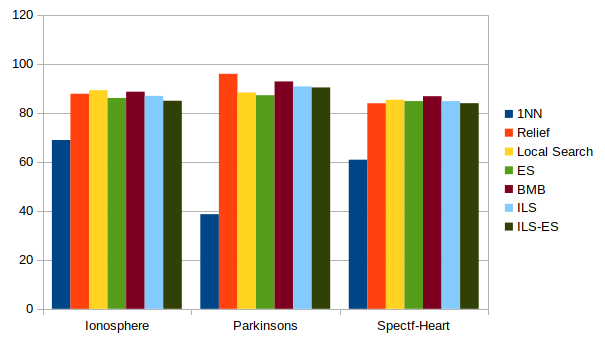
\includegraphics[width=0.65\textwidth]{images/tasa_clas.png}
		\caption{Tasa de clasificación.}
	\end{figure}

	Se observa que, a parte de 1NN, el resto de algoritmos proporcionan tasas de clasificación similares entre sí, dependiendo del dataset ganan unos u otros, no hay un patrón claro. Aunque Relief da buen resultado tampoco es de mucho interés pues sabemos que no proporciona apenas tasa de reducción. Lo que sí podemos destacar es que los algoritmos basados en trayectorias múltiples han dado resultados muy competitivos con BL, de hecho marcan nuevos máximos en Parkinsons y Spect-Heart. BMB destaca en todos los casos frente a ILS e ILS-ES, además ILS también da mejores tasas que ILS-ES. Por otra parte el algoritmo basado en trayectoria simple, ES, no ha superado a BL en ningún dataset aunque sí da valores cercanos, en Ionosphere y Spect-Heart supera a ILS-ES y queda cerca de ILS.~\\
	
	
	Vemos ahora las tasas de reducción:

	\begin{figure}[H]
		\centering
		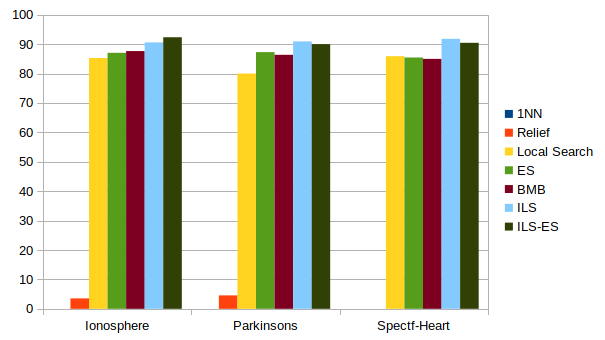
\includegraphics[width=0.65\textwidth]{images/tasa_red.png}
		\caption{Tasa de reducción.}
	\end{figure}
	
	BL era el que mejor resultado proporcionaba en los algoritmos de referencia. Vemos que se han mejorado los resultados en los 3 datasets. Los máximos los marcan los algoritmos de trayectorias múltiples ILS e ILS-ES, aunque ILS con enfriamiento simulado solo a superado a ILS (con BL) en Ionosphere. También cabe destacar que ES, a pesar de ser de trayectoria simple, ha dado tasas de reducción equiparables a BMB, incluso mejores tanto en Parkinsons y Spect-Heart. ~\\
	
	Mostramos también los tiempos de ejecución a los que se hará mención:
	
	\begin{figure}[H]
		\centering
		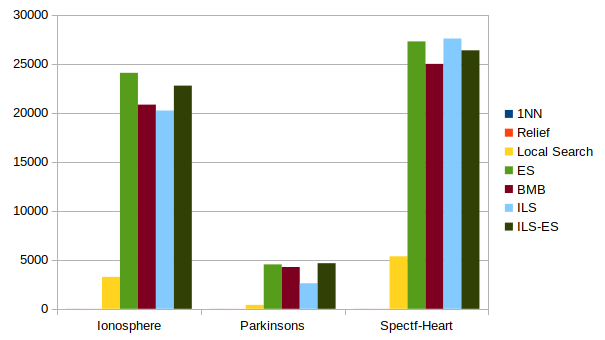
\includegraphics[width=0.65\textwidth]{images/tiempos.png}
		\caption{Tiempos de ejecución.}
	\end{figure}
	
	Por último el valor agregado:
	\begin{figure}[H]
		\centering
		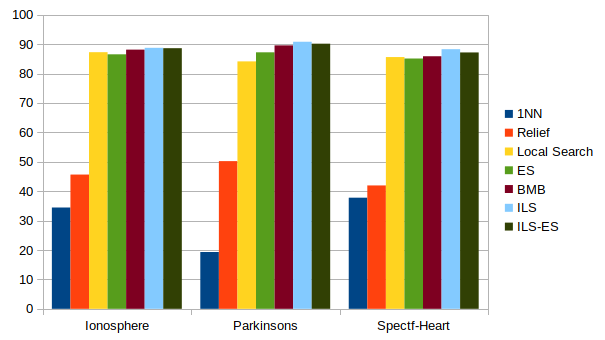
\includegraphics[width=0.65\textwidth]{images/tasa_agr.png}
		\caption{Valor de función objetivo o agregado.}
	\end{figure}

	
	De nuevo se han marcado nuevos máximos respecto a los resultados de BL en los 3 datasets. Los mejores resultados vienen dados por los algoritmos basados en trayectorias múltiples, siendo el mejor ILS en los 3 datasets. El segundo mejor algoritmo ha sido ILS-ES (en los 3 datasets). La búsqueda local iterativa ha resultado ser la estrategia que mayor fitness proporciona. En tercer lugar encontramos BMB (en los 3 datasets), otra técnica de trayectoria múltiple, que sigue siendo mejor que las estrategias de trayectorias simples. Entre los algoritmos de trayectorias simples encontramos resultados similares y competidos; en Ionosphere y Spect-Heart gana BL, y en Parkinsons gana ES, no hay un ganador consistente.\\
	
	Se comparan las técnicas según tipología:\\
	
	
	\underline{Trayectorias simples contra trayectorias múltiples}
	
	Como podemos ver, los algoritmos basados en trayectorias múltiples (BMB, ILS, ILS-ES) proporcionan un fitness mayor a los de trayectorias simples (BL y ES).
	
	Lo anterior puede comprobarse con BL vs BMB, BL vs ILS, y ES vs ILS-ES. En todos los casos ganan las estrategias de trayectorias múltiples que introducen más diversidad de soluciones.
	
	Lo que se observa por tanto es que da mejor resultado intentar, para un mismo número de evaluaciones de función objetivo, diversificar esas evaluaciones en varias BLs o ESs y explorar varios máximos locales, sin explotarlos demasiado, que invertir todas las evaluaciones en explotar un máximo que aunque se alcance puede nos ser tan bueno.\\
	
	\underline{BMB contra ILS}
	
	Vemos que ILS ha dado mejor tasa agregada que BMB en los 3 datasets. 
	
	Esto es, ha dado mejor resultado partir de una solución con buen fitness (ya aplicada una BL) e ir realizando mutaciones fuertes que partir de soluciones aleatorias independientes como en el caso de BMB.
	
	También cabe mencionar que BMB requiere generar 15 soluciones aleatorias lo cual juega en contra de su tiempo de ejecución, sin embargo no ha supuesto gran diferencia con ILS pues en la implementación de ILS también se ha requerido elegir aleatoriamente las componentes a mutar, de hecho da mayor tiempo de ejecución en Spect-Heart.\\
	
	\underline{BL contra ES}
	
	Podemos ver que se han obtenido tasas agregadas muy similares entre BL y ES, siendo ligeramente mejor BL en Ionosphere y Spectf-Heart. Cabe destacar que BL ha requerido además mucho menos tiempo de ejecución, esto tiene sentido pues, a diferencia de ES, no requiere generar soluciones aleatorias.
	
	Además sabemos que ES acepta soluciones peores a la actual, aumentando así la capacidad de exploración. Es decir, dependiendo del dataset y los óptimos locales que se tengan puede ser más efectivo introducir más exploración con ES o buscar más explotación con BL; esto podría explicar que en Parkinsons se obtenga mejor resultado con ES, aunque siempre hay una componente de aleatoriedad.
	
	Lo anterior también se aplica a ILS y ILS-ES, donde se han obtenido resultados similares aunque ligeramente mejores a favor de ILS.
	\iffalse
	En cuanto a los tiempos de ejecución:
	
	\begin{figure}[H]
		\centering
		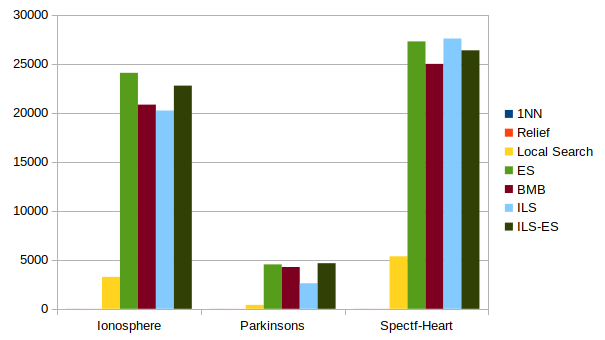
\includegraphics[width=0.65\textwidth]{images/tiempos.png}
		\caption{Tiempos.}
	\end{figure}
	
	Anteriormente BL era el algoritmo con mayor tiempo de ejecución. Ahora observamos una gran diferencia respecto BL: los algoritmos generacionales y meméticos suponen más de 4 veces el tiempo de BL, se ha requerido mucho tiempo para mejorar, y no por mucho, al resultado de BL. Los algoritmos genéticos tienen tiempos de ejecución similares entre sí. Sí se observa mayor tiempo de ejecución de los algoritmos meméticos respecto a genéticos ya que, aunque realizan las mismas evaluaciones de función objetivo, tienen como ``añadido'' las operaciones de la búsqueda local.~\\
		\fi

\end{document}
	

